\section{Results}
\label{sec:flakycat-resuts}

\subsection{RQ1: How effective is FlakyCat compared to approaches based on other combination of test representation and classifier? } 

\begin{table*}[htbp]
\caption{Comparing performances of FlakyCat (CodeBERT and Few-Shot Learning) with traditional machine learning classifiers}
\centering
\begin{tabular}{|c|c|c|c|c|c|c|c|c|c|c|c|c|c|c|c|}
\hline
\textbf{Model} & \multicolumn{5}{|c|}{\textbf{Smells-based}} & \multicolumn{5}{|c|}{\textbf{Vocabulary-based}} &\multicolumn{5}{|c|}{\textbf{CodeBERT-based}} \\
\cline{2-16} 
\textbf{} & \textbf{\textit{Precision}}& \textbf{\textit{Recall}} & \textbf{\textit{ MCC}}& \textbf{\textit{F1}} & \textbf{\textit{AUC}}& \textbf{\textit{Precision}}& \textbf{\textit{Recall}} & \textbf{\textit{ MCC}}& \textbf{\textit{F1}} & \textbf{\textit{AUC}} & \textbf{\textit{Precision}}& \textbf{\textit{Recall}} &\textbf{\textit{ MCC}}& \textbf{\textit{F1}} & \textbf{\textit{AUC}}\\
\hline


SVM & 0.11 & 0.34 & 0.00 & 0.17 & 0.50
& 0.61 & 0.52 & 0.37 & 0.45 & 0.66 
& 0.27 & 0.43 & 0.22 & 0.33 & 0.60 \\

\hline

KNN & 0.24 & 0.37 & 0.11 & 0.29 & 0.55
& 0.44 & 0.48 & 0.31 & 0.45 & 0.65 
& 0.56 & 0.53 & 0.37 & 0.51 & 0.68 \\

\hline

DT & 0.31 & 0.33 & 0.10 & 0.23 & 0.53 
& 0.53 & 0.53 & 0.39 & 0.52 & 0.69
& 0.49 & 0.50 & 0.34 & 0.49 & 0.67 \\

\hline

RF & 0.32 & 0.34 & 0.12 & 0.24 & 0.54
& 0.72 & 0.61 & 0.49 & 0.56 & 0.72 
& 0.68 & 0.66 & 0.55 & 0.62 & 0.76 \\

\hline
\textbf{FSL} & 0.13 & 0.18 & -0.01 & 0.13 & 0.50 
& 0.69 & 0.68 & 0.58 & 0.67 & 0.79
& \textbf{0.74} &\textbf{0.73} & \textbf{0.65} & \textbf{0.73} & \textbf{0.83} \\
\hline
\end{tabular}
\label{scores}
\vspace{-5mm}
\end{table*}

Following the outlined experimental design, we trained and tested FlakyCat and the four traditional classifiers, using the three source code representations, the vectors obtained from CodeBERT, the vectors based on vocabulary, and the ones based on test smells. The obtained results are presented in Table~\ref{scores}. The results show that FlakyCat achieves the best performance for all evaluation metrics. 
It obtained an average weighted F1 score of 73\% and a precision of 74\%.
We get an MCC of 0.65 (bounds for this metric are between -1 and 1), being close to 1 means a perfect classification. Finally, the AUC of 0.83 shows that the model is able to distinguish flaky tests from different classes. 

\paragraph{Representation effect}
Regarding the three code representations, CodeBERT achieves the best performance for RF, KNN, and FSL, with an F1 score between 0.51 and 0.73 for the three classifiers. 
When using the vocabulary-based vectors, SVM and DT perform better than using CodeBERT. With this representation, all classifiers do not exceed an F1 score of 0.67.
The representation based on test smells yields lower results, with the best F1 score being 0.29.
The CodeBERT representation seems then promising to use when learning to classify flaky tests according to their categories. 

\paragraph{Classifier effect}
Regarding the choice of classifier, we find that the FSL classifier based on similarity achieves the best performance using the representations based on CodeBERT and vocabulary. Among traditional classifiers, Random Forest obtains the best results, as reported in previous flaky test classification studies~\cite{Pinto2020,Haben2021}. Classifiers relying on the smell-based representation have more difficulty to classify flaky tests. Using this code representation, the KNN classifier achieved the best F1 score: 0.29. Two categories had a positive impact to achieve this score: \textit{Async wait}, and \textit{Test order dependency}. This can be explained by the presence of test smells strongly related to these two categories, including Sleepy test and Resource optimism. Other flakiness categories seem to be more challenging to predict using existing test smells. 

\paragraph{Random-guessing comparison}
In the previous paragraph, we compared different models and different code representations and saw that FlakyCat gave the best results. Because all the existing approaches were designed to detect flaky tests from non-flaky tests, they might not be suitable for the specific task of classifying flaky tests according to their categories. As no other category-based classification technique exist so far, we show the performance of a random guesser as another baseline. We consider two random guessing approaches, the first one where we randomly affect a class to each flaky test and the second one where we weigh the random affectation according to the prevalence of flaky tests in each category. Both approaches are considered as the dataset balance might be different from the one found in various projects. Results are listed in Table ~\ref{scores-random}. F1 scores for Random and Weighted Random are respectively of 0.21 and 0.25. With an F1 score of 0.73, we see that FlakyCat performs better than the two considered random-guessing approaches. 

\begin{tcolorbox}

\textbf{RQ1} Overall, our results show that automatic classification of flaky test categories with a limited amount of data is a challenging but feasible and promising task. 
% it is possible to automatically classify flaky test categories with a limited amount of data. 
The representation based on CodeBERT gives better results compared to the ones based on test smells and vocabulary. We also found that Few Shot Learning performs better than traditional machine learning classifiers. 

\end{tcolorbox}

\begin{table}[ht]
\caption{Performance of random guessing approach}
\centering
\begin{tabular}{|c|c|c|c|c|c|}
\hline
\textbf{Method} & \textbf{\textit{Precision}}& \textbf{\textit{Recall}} & \textbf{\textit{ MCC}}& \textbf{\textit{F1}} & \textbf{\textit{AUC}} \\
\hline
Random & 0.25 & 0.20 & -0.01 & 0.21 & 0.50 \\
\hline
Weighted Random & 0.25 & 0.26 & 0.02 & 0.25 & 0.51 \\
\hline
\end{tabular}
\label{scores-random}
\end{table}

\subsection{RQ2: How effective is FlakyCat in predicting each of the considered flakiness categories?}

\begin{figure}[htbp]
\centering
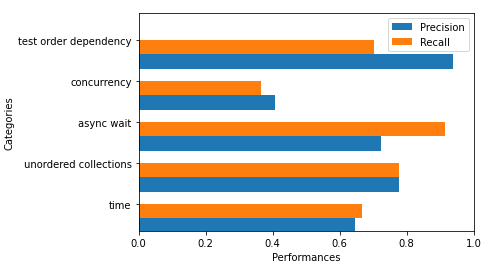
\includegraphics[scale=0.8]{figures/flakycat/FSL.PNG}
\caption{Precision and Recall per flakiness category using FlakyCat}
\label{fig:FSL}
\end{figure}

Figure~\ref{fig:FSL} shows performances achieved by FlakyCat for each of the five flakiness categories. Results show that the category \textit{Async wait} is the easiest for the model to classify, with an F1 score of 0.81. The category \textit{Test order dependency}, \textit{Unordered collections} and \textit{Time} respectively have an F1 score of 0.80, 0.78 and 0.66. \textit{Concurrency} performances are lower with an F1 score of 0.39. 
We suspect that concurrency issues happen in many cases in the code under test. As FlakyCat only relies on the test source code, this would indeed explain why performances are lower in this case. Another supposition is that concurrency issues and asynchronous waits are sometimes closely related. We discuss an example of this in Section~\ref{sec:discussion:reasoning}. \\




%\begin{table}[htbp]
%\caption{Performances by categories using FlakyCat}
%\begin{center}
%\begin{tabular}{|c|c|c|c|}
%\hline

% the scores avg for the cross validation 

%\textbf{Category} & \textbf{\textit{Precision}}& \textbf{\textit{ Recall}} & \textbf{\textit{Weighted F1-score}} \\
%\hline
%Unordered collections & 0.78 & 0.78 & 0.78 \\
%\hline
%test order dependency & 0.94 & 0.70 & 0.80 \\
%\hline
%Async waits & 0.72 & 0.92 & 0.81 \\
%\hline
%Time & 0.65 & 0.67 & 0.66 \\
%\hline
%Concurrency & 0.41 & 0.37 & 0.39 \\
%\hline
%\end{tabular}
%\label{tab_classes}
%\end{center}
%\end{table}

\begin{tcolorbox}

\textbf{RQ2} While the four flakiness categories \textit{Async waits}, \textit{Test order dependency}, \textit{Unordered collections},  and \textit{Time} show good ability to be detected automatically, \textit{Concurrency} remains difficult to detect by relying only on the test case code. 

\end{tcolorbox}

\begin{table*}[htbp]
\caption{Prevalence of different types of statements in each flakiness category for true positive predictions }
\centering
\resizebox{\textwidth}{!}{
\begin{tabular}{|c|c|c|c|c|c|c|c|c|c|c|}
\hline
 & \#Statements &	Control flow &	Constants &	Asserts &	Threads	& Waits &	Network & Global variables &	Usage of Date/time	 & I/O \\
\hline 
Async Waits & 80 &	16,25\% &	55\%   &	20\%	& 20\% &	27,5\% &	25\% &	11,25\% & 	3,75\% & 	6,25\% \\

\hline 
Concurrency & 34 &	23,53\% &	47,06\% &	17,65\% &	29,41\% &	14,70\% &	14,70\% &	5,88\% &	17,65\% & 2,94\%  \\
\hline 

Test order dependency & 69 &	8,69\% &	60,87\% &	13,04\% & 0\% &	4,35\% &	8,69\% &	2,90\% &	7,25\% &	47,82\% \\

\hline 

Time & 32 &	18,75\% &	56,25\% &	50\%	& 0\%	& 0\% & 	0\% &	9,375\% &	62,5\% &	6,25\% \\
\hline 

Unordered collections & 42 &	4,76\% &	66,67\% &	38,09\% &	0\% &	0\% &	2,38\% &	4,76\% &	0\% & 4,76\%  \\
\hline
\end{tabular}
}
\label{TabStatments}
\vspace{-5mm}
\end{table*}

\subsection{RQ3: How do statements of the test code influence the
predictions of FlakyCat?}

Table~\ref{TabStatments} reports the prevalence (\%) of the different types of statements among all influential statements per flakiness category, \eg 100\% Asserts in the \textit{Time} category would mean that all influential statements for the \textit{Time} category contain assert statements. 

Compared to other flakiness categories, the percentage of assertions in the influential statements of \textit{Time} and \textit{Unordered collections} is high, 50\% and 38.09\% respectively. Based on our analysis, this includes in particular assertions that perform exact comparisons, such as \texttt{assertEquals()}, between constant values and collection items, or dates for example. 
29,41\% of influential statements in the \textit{Concurrency} category include thread manipulation, and 20\% for the \textit{Async Waits} category, while the rest of the categories have none. 
Statements containing explicit waits represent respectively 27,5\% and 14,7\% for \textit{Async Waits} and \textit{Concurrency} categories, but below 5\% for \textit{Test order dependency} and zero for the others. Statements containing date or time values are most common in the \textit{Time} category with 62,5\%. We note that they appear as well in a small proportion, 17,65\%, for \textit{Concurrency}. Statements from the I/O calls group are mainly found in the \textit{Test order dependency}.
For \textit{Control flow}, \textit{Constants}, and \textit{Global variables} statements are almost evenly distributed. We include a spreadsheet containing all statements analyzed in our replication package. 

% The results show that FlakyCat is able to differentiate between the features that are important to each flakiness category by considering the correlation between the types of statements and flakiness categories. This also suggests that CodeBERT is able to grasp some semantics from the test code. \\

\vspace{2mm}
\begin{tcolorbox}
\textbf{RQ3} The interpretability technique we presented enable us to find which statements impact FlakyCat's decision. We also find hints that specific flakiness categories have distinct statement types (\eg Usage of Date/time for the \textit{Time} category) while some others have similar prevalence (\eg Threads for \textit{Async Waits} and \textit{Concurrency} categories).
By highlighting these statements, our interpretability technique may provide information to developers to better understand flaky tests, their categories and their causes.
\end{tcolorbox}

% asserts -> Time & unordered collections
% New instance & constants -> same distribution across categories
% time -> mostly time but also async waits and concurrency ( not for collections )
% threads & waits -> only async waits and concurrency
% external API calls -> mainly Async waits & concurrency

% 1. model learnt what needs to be learnt and Codebert learns good features 
% 2. 

